\documentclass[aspectratio=169, table]{beamer}

\usepackage[utf8]{inputenc}
\usepackage{listings} 

\usepackage{tikz}
\usetikzlibrary{arrows.meta, positioning, shapes.geometric, calc}

\usetheme{Pradita}

\subtitle{IF140303-Web Application Development}

\title{Session-10:\\
\Huge{
GitHub OAuth:\\in Phoenix\\
\vspace{-20pt}
}
}
\date[Serial]{\scriptsize{PRU/SPMI/FR-BM-18/0222}}
\author[Pradita]{\small{\textbf{Alfa Yohannis}}}

\lstdefinelanguage{Elixir} {
	keywords={def, defmodule, do, end, for, if, else, true, false, scope},
	language=ruby,
	basicstyle=\ttfamily\small,
	keywordstyle=\color{blue}\bfseries,
	ndkeywords={@spec, @moduledoc, iex, Enum, @doc, add, alter, field, has_many, timestamps},
	ndkeywordstyle=\color{purple}\bfseries,
	sensitive=true,
	commentstyle=\color{gray},
	stringstyle=\color{red},
	numbers=left,
	numberstyle=\tiny\color{gray},
	breaklines=true,
	frame=lines,
	backgroundcolor=\color{lightgray!10},
	tabsize=2,
	comment=[l]{\#},
	morecomment=[s]{/*}{*/},
	commentstyle=\color{gray}\ttfamily,
	stringstyle=\color{purple}\ttfamily,
	showstringspaces=false
}


\lstdefinelanguage{bash} {
	keywords={},
	basicstyle=\ttfamily\small,
	keywordstyle=\color{blue}\bfseries,
	ndkeywords={iex},
	ndkeywordstyle=\color{purple}\bfseries,
	sensitive=true,
	commentstyle=\color{gray},
	stringstyle=\color{red},
	numbers=left,
	numberstyle=\tiny\color{gray},
	breaklines=true,
	frame=lines,
	backgroundcolor=\color{lightgray!10},
	tabsize=2,
	comment=[l]{\#},
	morecomment=[s]{/*}{*/},
	commentstyle=\color{gray}\ttfamily,
	stringstyle=\color{purple}\ttfamily,
	showstringspaces=false
}

\lstdefinelanguage{html} {
	keywords={h1, b, a, href, class},
	basicstyle=\ttfamily\small,
	keywordstyle=\color{blue}\bfseries,
	ndkeywords={p, else, if, do, end},
	ndkeywordstyle=\color{purple}\bfseries,
	sensitive=true,
	commentstyle=\color{gray},
	stringstyle=\color{red},
	numbers=left,
	numberstyle=\tiny\color{gray},
	breaklines=true,
	frame=lines,
	backgroundcolor=\color{lightgray!10},
	commentstyle=\color{gray}\ttfamily,
	stringstyle=\color{purple}\ttfamily,
	morecomment=[s]{<!--}{-->},
	string=[s]{'}{'},
	morestring=[s]{"}{"},
	tabsize=2
}


\begin{document}
	
	\frame{\titlepage}
	
		\begin{frame}[fragile]
		\frametitle{Contents}
		\vspace{20pt}
		\begin{columns}[t]
			\column{0.5\textwidth}
			\tableofcontents[sections={1-6}]
			
			\column{0.5\textwidth}
			\tableofcontents[sections={7-99}]
		\end{columns}
	\end{frame}


\section{Introduction}

\begin{frame}{GitHub OAuth in Phoenix}
\vspace{20pt}
\begin{itemize}
  \item OAuth lets applications verify user identity without handling passwords directly.
  \item Users grant permission to providers (e.g., GitHub) to share basic profile data securely.
  \item This reduces security risks and improves usability: users sign in without creating new accounts.
  \item In Phoenix, OAuth integration is simplified using the \texttt{Ueberauth} library.
  \item \texttt{ueberauth\_github} provides “Login with GitHub” support following modern web best practices.
\end{itemize}
\end{frame}

\section{How OAuth Works}

% =============================
% FRAME 1 — TIKZ DIAGRAM
% =============================
\begin{frame}{OAuth Authorization Code Flow}
\centering
\vspace{25pt}

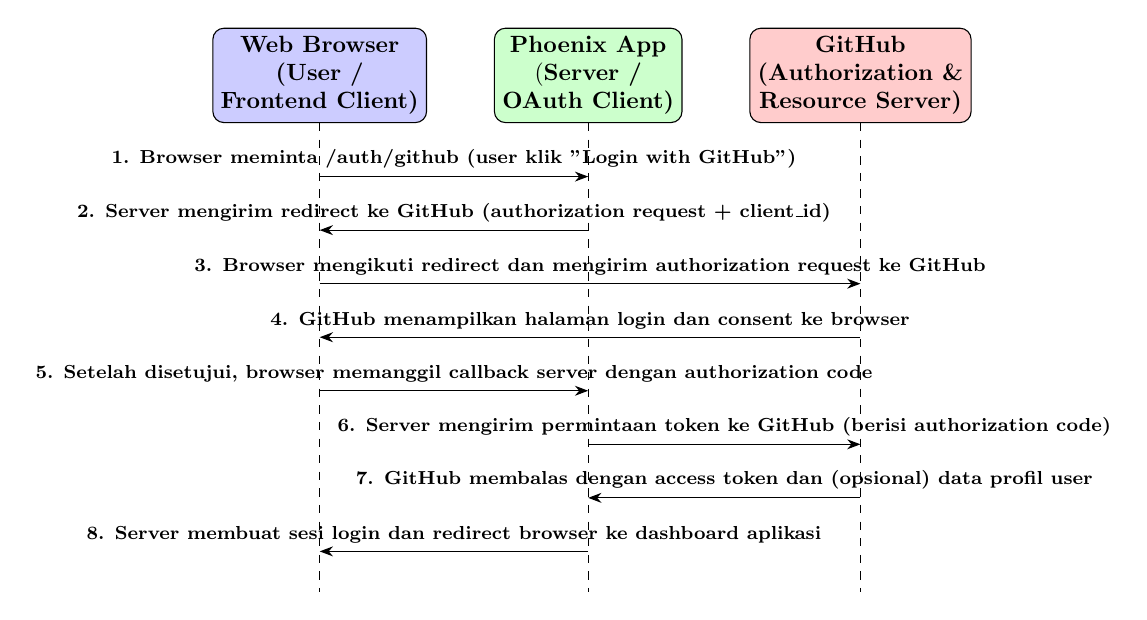
\begin{tikzpicture}[
    scale=0.85,
    transform shape,
    >=Stealth,
    node distance=1cm,
    actor/.style={
      rectangle,
      draw,
      rounded corners,
      minimum width=1cm,
      minimum height=1cm,
      align=center
    },
    seq/.style={font=\footnotesize}
]

% Tiga aktor utama
\node[actor, fill=blue!20] (browser) {\textbf{Web Browser}\\\textbf{(User /}\\\textbf{Frontend Client)}};
\node[actor, right=of browser, fill=green!20] (server) {\textbf{Phoenix App}\\(\textbf{Server /} \\\textbf{OAuth Client)}};
\node[actor, right=of server, fill=red!20] (github) {\textbf{GitHub}\\\textbf{(Authorization \&} \\\textbf{Resource Server)}};

% Lifeline (garis putus-putus ke bawah)
\draw[dashed] (browser.south) -- ($(browser.south)+(0,-7)$);
\draw[dashed] (server.south)  -- ($(server.south)+(0,-7)$);
\draw[dashed] (github.south)  -- ($(github.south)+(0,-7)$);

% Koordinat langkah (vertikal)
\coordinate (b1) at ($(browser.south)+(0,-0.8)$);
\coordinate (s1) at ($(server.south) +(0,-0.8)$);

\coordinate (b2) at ($(browser.south)+(0,-1.6)$);
\coordinate (s2) at ($(server.south) +(0,-1.6)$);

\coordinate (b3) at ($(browser.south)+(0,-2.4)$);
\coordinate (g3) at ($(github.south) +(0,-2.4)$);

\coordinate (b4) at ($(browser.south)+(0,-3.2)$);
\coordinate (g4) at ($(github.south) +(0,-3.2)$);

\coordinate (b5) at ($(browser.south)+(0,-4.0)$);
\coordinate (s5) at ($(server.south) +(0,-4.0)$);

\coordinate (s6) at ($(server.south) +(0,-4.8)$);
\coordinate (g6) at ($(github.south) +(0,-4.8)$);

\coordinate (s7) at ($(server.south) +(0,-5.6)$);
\coordinate (g7) at ($(github.south) +(0,-5.6)$);

\coordinate (s8) at ($(server.south) +(0,-6.4)$);
\coordinate (b8) at ($(browser.south)+(0,-6.4)$);

% 1. Browser -> Server
\draw[->] (b1) -- (s1)
  node[midway, above, seq]{\textbf{1. Browser meminta /auth/github (user klik "Login with GitHub")}};

% 2. Server -> Browser
\draw[->] (s2) -- (b2)
  node[midway, above, seq]{\textbf{2. Server mengirim redirect ke GitHub (authorization request + client\_id)}};

% 3. Browser -> GitHub
\draw[->] (b3) -- (g3)
  node[midway, above, seq]{\textbf{3. Browser mengikuti redirect dan mengirim authorization request ke GitHub}};

% 4. GitHub -> Browser
\draw[->] (g4) -- (b4)
  node[midway, above, seq]{\textbf{4. GitHub menampilkan halaman login dan consent ke browser}};

% 5. Browser -> Server
\draw[->] (b5) -- (s5)
  node[midway, above, seq]{\textbf{5. Setelah disetujui, browser memanggil callback server dengan authorization code}};

% 6. Server -> GitHub
\draw[->] (s6) -- (g6)
  node[midway, above, seq]{\textbf{6. Server mengirim permintaan token ke GitHub (berisi authorization code)}};

% 7. GitHub -> Server
\draw[->] (g7) -- (s7)
  node[midway, above, seq]{\textbf{7. GitHub membalas dengan access token dan (opsional) data profil user}};

% 8. Server -> Browser
\draw[->] (s8) -- (b8)
  node[midway, above, seq]{\textbf{8. Server membuat sesi login dan redirect browser ke dashboard aplikasi}};

\end{tikzpicture}

\end{frame}




% =============================
% FRAME 2 — EXPLANATION
% =============================
\begin{frame}{How OAuth Works}
\vspace{20pt}
\begin{itemize}
  \item OAuth 2.0 involves the browser, Phoenix server, and GitHub as authorization/resource server.
  \item The browser is redirected to GitHub for login and permission.
  \item GitHub returns an authorization code to Phoenix via callback.
  \item Phoenix securely exchanges the code for an access token using a server-to-server request.
  \item The token allows Phoenix to fetch the user’s GitHub profile without ever handling passwords.
\end{itemize}
\end{frame}

\section{Migration}

\begin{frame}[fragile]{Creating the Users Table (Migration)}
\vspace{30pt}
The application requires a \texttt{users} table to store GitHub OAuth login data, including email, provider name, and access token.
This migration file is placed inside \texttt{priv/repo/migrations/} and defines the necessary database structure.

\begin{lstlisting}[language=Elixir, basicstyle=\ttfamily\scriptsize]
defmodule Hiwi.Repo.Migrations.AddUsers do
  use Ecto.Migration

  def change do
    create table(:users) do
      add :email, :string
      add :provider, :string
      add :token, :string
      timestamps()
    end
  end
end
\end{lstlisting}

\begin{lstlisting}[language=bash, basicstyle=\ttfamily\scriptsize]
mix ecto.migrate
== Running 20251102090628 Hiwi.Repo.Migrations.AddUsers.change/0 forward
== Migrated 20251102090628 in 0.03s
\end{lstlisting}

\end{frame}

\section{Model}

%==========================
% FRAME 1 — CODE ONLY
%==========================
\begin{frame}[fragile]{User Schema (Model)}
\vspace{15pt}

\begin{lstlisting}[language=Elixir, basicstyle=\ttfamily\scriptsize]
defmodule Hiwi.User do
  use Ecto.Schema
  import Ecto.Changeset

  schema "users" do
    field :email, :string
    field :provider, :string
    field :token, :string
    timestamps(type: :utc_datetime)
  end

  def changeset(user, attrs) do
    user
    |> cast(attrs, [:email, :provider, :token])
    |> validate_required([:email, :provider, :token])
  end
end
\end{lstlisting}

\end{frame}

%==========================
% FRAME 2 — EXPLANATION ONLY
%==========================
\begin{frame}{Model Explanation}
\vspace{20pt}

\begin{itemize}
  \item The \texttt{Hiwi.User} schema represents the \texttt{users} table created by the migration, defining the fields used to store GitHub OAuth login data.
  \item The schema includes three main fields: \texttt{email}, \texttt{provider}, and \texttt{token}, each mapped directly to database columns.
  \item The \texttt{timestamps/1} macro automatically generates \texttt{inserted\_at} and \texttt{updated\_at} columns with UTC datetime.
  \item The \texttt{changeset/2} function validates incoming data, casts only allowed fields, and ensures required values are present before inserting or updating records.
  \item This schema can be extended later with additional GitHub fields such as \texttt{name}, \texttt{avatar\_url}, or \texttt{github\_id} as the application grows.
\end{itemize}

\end{frame}


\section{Dependencies}

%========================================
% FRAME 1 — CODE ONLY
%========================================
\begin{frame}[fragile]{Ueberauth Dependencies in mix.exs}
\vspace{10pt}

\begin{columns}[T]

%---------------- LEFT COLUMN ----------------
\begin{column}{0.75\textwidth}

\begin{lstlisting}[language=Elixir, basicstyle=\ttfamily\scriptsize]
defmodule Hiwi.MixProject do
  use Mix.Project

  def application do
    [
      mod: {Hiwi.Application, []},
      extra_applications: [ logger, :runtime_tools, :ueberauth, :ueberauth_github ]
    ]
  end

  defp deps do
    [
      # OAuth dependencies
      {:ueberauth, "~> 0.10"}, {:ueberauth_github, "~> 0.8.3"}
    ]
  end
end
\end{lstlisting}

\end{column}

%---------------- RIGHT COLUMN ----------------
\begin{column}{0.20\textwidth}

\begin{lstlisting}[language=bash, basicstyle=\ttfamily\scriptsize]
mix deps.get
mix compile
\end{lstlisting}
\textbf{Ueberauth:} \url{https://github.com/ueberauth/ueberauth}\\
\vspace{5pt}
\textbf{GitHub:} \url{https://github.com/ueberauth/ueberauth_github}
\end{column}

\end{columns}

\end{frame}


%========================================
% FRAME 2 — EXPLANATION ONLY
%========================================
\begin{frame}{Dependencies Explanation}
\vspace{20pt}

\begin{itemize}
  \item Phoenix uses the \texttt{Ueberauth} ecosystem to support authentication through external providers such as GitHub, Google, or Facebook.
  \item The \texttt{ueberauth\_github} strategy implements GitHub’s OAuth 2.0 flow, handling authorization URLs, token exchange, and user profile retrieval.
  \item Both \texttt{:ueberauth} and \texttt{:ueberauth\_github} must be added to the \texttt{deps} list and to the \texttt{extra\_applications} list so they run as part of the OTP application.
  \item After updating \texttt{mix.exs}, running \texttt{mix deps.get} and \texttt{mix compile} downloads and builds the required libraries.
  \item With dependencies installed, the next step is configuring GitHub OAuth in \texttt{config/config.exs} and adding the routes \texttt{/auth/github} and \texttt{/auth/github/callback}.
\end{itemize}

\end{frame}

\section{GitHub}

\begin{frame}{Creating a GitHub OAuth App}
\vspace{15pt}

\begin{itemize}
  \item Log in to your GitHub account.
  \item Open:
    \texttt{Settings $\rightarrow$ Developer Settings $\rightarrow$ OAuth Apps}
  \item Click \textbf{New OAuth App}.
  \item Fill in the required fields:
    \begin{itemize}
      \item Application Name: \texttt{Hiwi}
      \item Homepage URL: \texttt{https://www.hiwi.com}
      \item Description: \texttt{Queue Management System}
      \item Callback URL: \texttt{http://localhost:4000/auth/github/callback}
    \end{itemize}
  \item Click \textbf{Register application}.
  \item Open the app again and click \textbf{Edit}.
  \item Copy the \textbf{Client ID}.
  \item Click \textbf{Generate a new client secret} and save it securely.
\end{itemize}

\end{frame}
%====================================================


%====================================================
\begin{frame}{GitHub OAuth App Output}
\vspace{20pt}

\begin{itemize}
  \item After registration you obtain:
  \begin{itemize}
    \item \textbf{GITHUB\_CLIENT\_ID}
    \item \textbf{GITHUB\_CLIENT\_SECRET}
  \end{itemize}

  \item These values must be added as environment variables.
  \item They will be read by Ueberauth to authenticate securely.
  \item The Client Secret is shown only once — store it safely.
\end{itemize}

\end{frame}
%====================================================

\section{Configuration}

\begin{frame}[fragile]{OAuth Configuration (config/config.exs)}
\vspace{15pt}

\begin{lstlisting}[language=Elixir, basicstyle=\ttfamily\scriptsize]
import Config

config :ueberauth, Ueberauth.Strategy.Github.OAuth,
  client_id: System.get_env("GITHUB_CLIENT_ID"),
  client_secret: System.get_env("GITHUB_CLIENT_SECRET")
\end{lstlisting}

\vspace{10pt}

\begin{itemize}
  \item Ueberauth reads GitHub OAuth credentials from environment variables.
  \item Storing secrets in the system environment prevents accidental exposure.
  \item Phoenix loads these values at runtime when handling OAuth requests.
\end{itemize}

\end{frame}

\section{Environment Variables}

\begin{frame}[fragile]{Environment Variables for GitHub OAuth}
\vspace{15pt}

\begin{lstlisting}[language=bash, basicstyle=\ttfamily\scriptsize]
$ nano ~/.bashrc

# GitHub OAuth
export GITHUB_CLIENT_ID="your_client_id"
export GITHUB_CLIENT_SECRET="your_client_secret"
\end{lstlisting}

\begin{lstlisting}[language=bash, basicstyle=\ttfamily\scriptsize]
$ source ~/.bashrc
\end{lstlisting}

\vspace{10pt}

\begin{itemize}
  \item Environment variables store secrets safely outside source code.
  \item Loaded by the shell before Phoenix runs.
  \item Ueberauth reads these values at runtime for secure OAuth authentication.
\end{itemize}

\end{frame}


%=====================================================
\section{View}
%=====================================================

%-----------------------------------------------------
% FRAME 1 — CODE
%-----------------------------------------------------
\begin{frame}[fragile]{View: Adding OAuth GitHub Button}
\vspace{15pt}

\begin{lstlisting}[language=html, basicstyle=\ttfamily\scriptsize]
<!-- lib/hiwi_web/components/layouts.ex -->
<li>
  <a href="http://localhost:4000/auth/github"
     class="btn btn-ghost">
    OAuth GitHub
  </a>
</li>

<li>
  <a href="https://phoenixframework.org/"
     class="btn btn-ghost">
    Website
  </a>
</li>
\end{lstlisting}

\end{frame}

%-----------------------------------------------------
% FRAME 2 — EXPLANATION
%-----------------------------------------------------
\begin{frame}{View: How the OAuth Button Works}
\vspace{15pt}

\begin{itemize}
  \item The button links to \texttt{/auth/github}, which starts the OAuth login flow.
  \item When clicked, Ueberauth redirects the browser to GitHub for authentication.
  \item CSS classes \texttt{btn btn-ghost} style the button (Tailwind/DaisyUI).
  \item This code lives in \texttt{layouts.ex}, making the button appear in the main navbar.
  \item After GitHub login, a callback to Phoenix completes the authentication.
\end{itemize}

\end{frame}

\section{Revoking Access / Logout}

\begin{frame}{Revoking Access / Logout}
\vspace{15pt}

\textbf{OAuth logout is more than deleting a local session.}  
GitHub may still hold valid access tokens, so users or administrators may need to revoke them for security reasons.

\begin{itemize}
  \item \textbf{Revoke for an individual user}  
    \begin{itemize}
      \item GitHub $\rightarrow$ Settings $\rightarrow$ Applications $\rightarrow$ Authorized OAuth Apps  
      \item Select the app $\rightarrow$ click \texttt{\vdots} $\rightarrow$ \textbf{Revoke}
      \item Token becomes invalid; the user must log in again.
    \end{itemize}

  \item \textbf{Revoke all user tokens (Admin-level)}  
    \begin{itemize}
      \item GitHub $\rightarrow$ Developer Settings $\rightarrow$ OAuth Apps  
      \item Select app $\rightarrow$ \textbf{Edit} $\rightarrow$ Revoke All User Tokens  
      \item All issued tokens become invalid globally.
    \end{itemize}

  \item \textbf{Effects on Phoenix App}  
    \begin{itemize}
      \item API calls with old tokens fail (Unauthorized).
      \item Phoenix can prompt re-login.
      \item Local session may still exist, but GitHub access is blocked.
    \end{itemize}
\end{itemize}

\end{frame}

\section{Router}

% ====================== FRAME 1 — CODE ======================
\begin{frame}[fragile]{Router: OAuth GitHub Routes}
\vspace{15pt}

\begin{lstlisting}[language=Elixir, basicstyle=\ttfamily\scriptsize]
#lib/hiwi\_web/router.ex
defmodule HiwiWeb.Router do
  use HiwiWeb, :router

  scope "/auth", HiwiWeb do
    pipe_through :browser

    # Start OAuth login
    get "/:provider", AuthController, :request

    # GitHub callback endpoint
    get "/:provider/callback", AuthController, :callback
  end
end
\end{lstlisting}

\begin{lstlisting}[language=bash, basicstyle=\ttfamily\scriptsize]
/auth/github
/auth/github/callback
http://localhost:4000/auth/github
http://localhost:4000/auth/github/callback
\end{lstlisting}

\end{frame}


% ====================== FRAME 2 — EXPLANATION ======================
\begin{frame}{Router Explanation}
\vspace{15pt}

\begin{itemize}
  \item All Phoenix routes are defined in \texttt{lib/hiwi\_web/router.ex}.
  \item The \textbf{/auth} scope groups all OAuth-related routes.
  \item \texttt{get "/:provider"}  
        Starts the OAuth login flow (e.g., \texttt{/auth/github}).
  \item \texttt{get "/:provider/callback"}  
        GitHub redirects here after user approval.
  \item Callback endpoint handles:
        \begin{itemize}
            \item reading the authorization code,
            \item exchanging it for an access token,
            \item fetching user profile data,
            \item creating a user session.
        \end{itemize}
  \item Must match the callback URL registered in GitHub OAuth App.
\end{itemize}

\end{frame}

\section{Controller}

\begin{frame}[fragile]{Controller 1}
\vspace{10pt}

\begin{columns}[T]  % Top alignment
%========================================
% LEFT COLUMN — CODE
%========================================
\begin{column}{0.55\textwidth}

\begin{lstlisting}[language=Elixir, basicstyle=\ttfamily\scriptsize]
# lib/hiwi_web/controllers/auth_controller.ex
defmodule HiwiWeb.AuthController do
  use HiwiWeb, :controller
  plug Ueberauth
  alias Hiwi.User
  alias Hiwi.Repo

  def callback(conn, params) do
    ...
  end

  defp signin(conn, changeset) do
    ...
  end

  defp insert_or_update_user(changeset) do
    ...
  end
end
\end{lstlisting}

\end{column}

%========================================
% RIGHT COLUMN — EXPLANATION
%========================================
\begin{column}{0.45\textwidth}

\begin{itemize}\small
  \item \textbf{HiwiWeb.AuthController} handles GitHub OAuth login logic.
  \item \textbf{plug Ueberauth} injects Ueberauth into requests under  
        \texttt{/auth/github} and \texttt{/auth/github/callback}.
  \item \textbf{callback/2} receives the GitHub response and parses  
        token + user profile.
  \item \textbf{signin/2} stores the session, sets flash messages, and redirects.
  \item \textbf{insert\_or\_update\_user/1} checks whether the user exists  
        and inserts or reuses the record.
  \item These functions together implement the full GitHub login workflow.
\end{itemize}

\end{column}

\end{columns}
\end{frame}


\begin{frame}[fragile]{Controller 2}
\begin{lstlisting}[language=Elixir, basicstyle=\ttfamily\scriptsize]
# lib/hiwi\_web/controllers/auth\_controller.ex
defmodule HiwiWeb.AuthController do
 ...
  def callback(conn, params) do
    IO.puts("conn = " <> Kernel.inspect(conn))
    IO.puts("conn: ")
    IO.inspect(conn)
    IO.puts("params = " <> Kernel.inspect(params))
    %{"code" => _code, "provider" => provider, "state" => _state} = params
    %{assigns: %{ueberauth_auth: auth}} = conn
    %{credentials: %{token: token}, info: %{email: email, nickname: nickname}} = auth

    user_params = %{
      token: token,
      email: email || nickname,
      provider: provider
    }

    IO.puts("user_params = " <> Kernel.inspect(user_params))

    changeset = User.changeset(%User{}, user_params)

    signin(conn, changeset)
  end
  ...
end
\end{lstlisting}
\end{frame}

\begin{frame}[fragile]{Controller 2 — Explanation}
\vspace{10pt}

\begin{columns}[T]
% ---------------- LEFT COLUMN ----------------
\begin{column}{0.48\textwidth}
\begin{itemize}\small
  \item The \textbf{callback/2} function executes after GitHub redirects to:
\begin{lstlisting}[language=bash, basicstyle=\ttfamily\scriptsize]
/auth/github/callback
\end{lstlisting}

  \item Debug output printed:
        \begin{itemize}
            \item full Plug.Conn
            \item callback params
        \end{itemize}

  \item OAuth data retrieved from:
\begin{lstlisting}[language=bash, basicstyle=\ttfamily\scriptsize]
conn.assigns.ueberauth_auth
\end{lstlisting}

  \item Extracted fields include:
        \begin{itemize}
            \item access token
            \item email / nickname
        \end{itemize}
\end{itemize}
\end{column}

% ---------------- RIGHT COLUMN ----------------
\begin{column}{0.48\textwidth}
\begin{itemize}\small
  \item The controller constructs:
\begin{lstlisting}[language=bash, basicstyle=\ttfamily\scriptsize]
user_params = %{
 token: token,
 email: email || nickname,
 provider: provider
}
\end{lstlisting}

  \item This is transformed into a changeset via:
\begin{lstlisting}[language=bash, basicstyle=\ttfamily\scriptsize]
User.changeset(%User{}, user_params)
\end{lstlisting}

  \item Finally, authentication flow continues:
\begin{lstlisting}[language=bash, basicstyle=\ttfamily\scriptsize]
signin(conn, changeset)
\end{lstlisting}

  \item This function inserts/loads the user and starts the session.
\end{itemize}
\end{column}

\end{columns}

\end{frame}




\begin{frame}[fragile]{Controller 3}
\vspace{20pt}
\begin{lstlisting}[language=Elixir, basicstyle=\ttfamily\scriptsize]
# lib/hiwi\_web/controllers/auth\_controller.ex
defmodule HiwiWeb.AuthController do
  ...
  defp signin(conn, changeset) do
    case insert_or_update_user(changeset) do
      {:ok, user} ->
        conn
        |> put_flash(:info, "Good to see you again!")
        |> put_session(:user_id, user.id)
        |> redirect(to: "/")

      {:error, reason} ->
        conn
        |> put_flash(:error, "Error when signing in: #{reason}")
        |> redirect(to: "/")
    end
  end
  ...
end
\end{lstlisting}
\end{frame}

\begin{frame}[fragile]{Controller 3 — Explanation}
\vspace{10pt}

\begin{columns}[T]
\begin{column}{0.48\textwidth}

\textbf{Successful Login}
\begin{itemize}\small
  \item Calls:
\begin{lstlisting}[language=bash, basicstyle=\ttfamily\scriptsize]
insert_or_update_user(...)
\end{lstlisting}
  \item If user exists or is inserted:
\begin{lstlisting}[language=bash, basicstyle=\ttfamily\scriptsize]
put_flash(:info, ...)
put_session(:user_id, user.id)
redirect("/")
\end{lstlisting}
\end{itemize}

\end{column}
\begin{column}{0.48\textwidth}

\textbf{Error Handling}
\begin{itemize}\small
  \item If database fails:
\begin{lstlisting}[language=bash, basicstyle=\ttfamily\scriptsize]
{:error, reason}
\end{lstlisting}
  \item Shows error flash  
  \item Redirects to home  
\end{itemize}

\textbf{Summary}
\begin{itemize}\small
  \item \texttt{signin/2} connects DB result → flash → redirect.
  \item Final step of OAuth login flow.
\end{itemize}

\end{column}
\end{columns}

\end{frame}



\begin{frame}[fragile]{Controller 4}
\vspace{20pt}
\begin{lstlisting}[language=Elixir, basicstyle=\ttfamily\scriptsize]
# lib/hiwi\_web/controllers/auth\_controller.ex
defmodule HiwiWeb.AuthController do
  ...
  defp insert_or_update_user(changeset) do
    case Repo.get_by(User, email: changeset.changes.email) do
      nil ->
        Repo.insert(changeset)

      user ->
        {:ok, user}
    end
  end
end
\end{lstlisting}
\end{frame}

\begin{frame}[fragile]{Controller 4 — Explanation}
\vspace{12pt}

\begin{columns}[T]
\begin{column}{0.48\textwidth}

\textbf{Purpose}
\begin{itemize}\small
  \item Handles saving or loading a user during OAuth login.
  \item Prevents duplicate users by checking the email first.
\end{itemize}

\textbf{Lookup Step}
\begin{lstlisting}[language=bash, basicstyle=\ttfamily\scriptsize]
Repo.get_by(User,
  email: changeset.changes.email)
\end{lstlisting}

\end{column}
\begin{column}{0.48\textwidth}

\textbf{Behavior}
\begin{itemize}\small
  \item If no user exists:
\begin{lstlisting}[language=bash, basicstyle=\ttfamily\scriptsize]
Repo.insert(changeset)
\end{lstlisting}

  \item If user already exists:
\begin{lstlisting}[language=bash, basicstyle=\ttfamily\scriptsize]
{:ok, user}
\end{lstlisting}

  \item Ensures OAuth login always returns a valid user struct.
\end{itemize}

\textbf{Summary}
\begin{itemize}\small
  \item Central logic for upsert-like user handling.
  \item Simplifies the login flow for both new and returning users.
\end{itemize}

\end{column}
\end{columns}

\end{frame}


\section{Demo}
\begin{frame}[fragile]{Demo: Testing GitHub OAuth Login}
\vspace{10pt}

\begin{columns}[T]
\begin{column}{0.48\textwidth}

\textbf{1. Start Phoenix Server}
\begin{lstlisting}[language=bash, basicstyle=\ttfamily\scriptsize]
mix phx.server
\end{lstlisting}

\textbf{2. Open App}
\begin{lstlisting}[language=bash, basicstyle=\ttfamily\scriptsize]
http://localhost:4000
\end{lstlisting}

\textbf{3. Click Login Button}
\begin{lstlisting}[language=bash, basicstyle=\ttfamily\scriptsize]
OAuth GitHub
\end{lstlisting}

\textbf{4. Redirect to GitHub}
\begin{lstlisting}[language=bash, basicstyle=\ttfamily\scriptsize]
/auth/github
\end{lstlisting}

\end{column}
\begin{column}{0.48\textwidth}

\textbf{5. Authorize App}
\begin{lstlisting}[language=bash, basicstyle=\ttfamily\scriptsize]
Authorize <username>
\end{lstlisting}

\textbf{6. Callback to Phoenix}
\begin{lstlisting}[language=bash, basicstyle=\ttfamily\scriptsize]
/auth/github/callback
\end{lstlisting}

\textbf{7. Success Flash}
\begin{lstlisting}[language=bash, basicstyle=\ttfamily\scriptsize]
Good to see you again!
\end{lstlisting}

\end{column}
\end{columns}

\end{frame}

\end{document}
